\section{Symbolic Representations for Natural Language}
\label{sec:bg:symbolic}
In the~\autoref{chap:intro}, we have listed serveral lexical,
syntactic and semantic structures in NLP. In this section, we will
mainly introduce more detailed background on the broad-coverage
semantic presentations~\S\ref{ssec:bg:broad-mr} and
application-specific representations on
dialogue~\S\ref{ssec:bg:dialogue-mr}.

Before we introduce each semantic representation, we first define the
term \kw{anchoring} and \kw{anchors}, and then we use them to organize
semantic representations in our dissertation.

\Paragraph{Anchoring} As the same definition of \kw{anchoring} used in the
Meaning Representation Parsing~(MRP) shared
task~\citep{Oep:Abe:Haj:19}, we distinguish different flavors of
semantic graphs based on the nature of the relationship they assume
between the linguistic surface signal~(typically a written sentence,
i.e. a string) and the nodes of the graph. We refer to this relation
as ~\kw{anchoring}~(of nodes onto sub-strings); other commonly used
terms include alignment, correspondence, or lexicalization.

\Paragraph{Anchor} Besides that, we also define the term~\kw{anchor} as
the surface substring in the sentence, which is \kw{anchoring} to the
corresponding node in the graph. According to the type of the
substring~(lexicon, phrase, sentence and so on), we mainly classify
the type of the \kw{anchors} into \kw{lexical-anchoring},
\kw{phrasal-anchoring} and
\kw{sentential-anchoring}.


\subsection{Broad-coverage Semantic Representation}
\label{ssec:bg:broad-mr}

For linguistic analysis, structures have been studied from
subword-level morphology ~\citep{beesley2003finite}, word-level
lexicon semantics~\citep{miller1998wordnet}, to single sentence
syntax/semantic
representations~\citep{baker1998berkeley,palmer2005proposition,collins2003head},
and multi-sentences discourse
analysis~\citep{carlson2003building,wolf2005representing,prasad2008penn}. A
broad-coverage semantic representation is a general-purpose meaning
representation language aiming to represent the multiple phenomena in
a single structure for broad-coverage text. This thesis covers
broad-coverage graph-based semantic representations in a single
sentence, which involves \kw{lexical-anchoring} and
\kw{phrasal-anchoring}. For lexical anchoring, we cover the DELPH-IN
MRS Bi-lexical Dependencies~\cite[DM,][]{ivanova2012did} and Prague
Semantic
Dependencies~\cite[PSD,][]{hajic2012announcing,miyao2014house},
Abstract Meaning Representation~\cite[AMR,][]{Ban:Bon:Cai:13}; While
for phrasal-anchoring, we study Universal Conceptual Cognitive
Annotation~\cite[UCCA,][]{Abe:Rap:13b}. The following lists a famous
sentence~(\#20001001 in MRP Corpus), which is also the first sentence
from WallStreetJournal~(WSJ) Corpus from the Penn
Treebank~\citep{Mar:San:Mar:93}.

\texttt{Pierre Vinken, 61 years old, will join the board as a nonexecutive director Nov.29.}

This sentence contains some interesting linguistic phenomes, such as
morphlogy words, person and date named entities. Taking it as an
example, we will introduce the detailed properties for each of the
representations.~\footnote{The summeriziation paper in MRP
  workshop~\citep{Mar:San:Mar:93} introduces another example-based
  comparative studies for different meaning representations.}

\subsubsection{Bi-lexical Semantic Dependencies}
\label{ssec:bg:bi-leixcal}

As shown in~\autoref{fig:intro-dog-dep}, syntactic dependency
structures captures the directed bi-lexical grammatical relations
between words. Each labeled arc represents a directed relation from
heads to dependents. However, different with the syntactic dependency
tree, semantic dependency graphs aims to represent the semantic
dependencies in the full sentence, inclduing word sense distinctions,
the reentrances for correference, predicate-argument structures in
semantic role labelling, namded entities representations and so
on. Because of the reentrances, semantic representations can be a
graph rather than a tree-like structures.
\begin{figure}[!th]
\centering
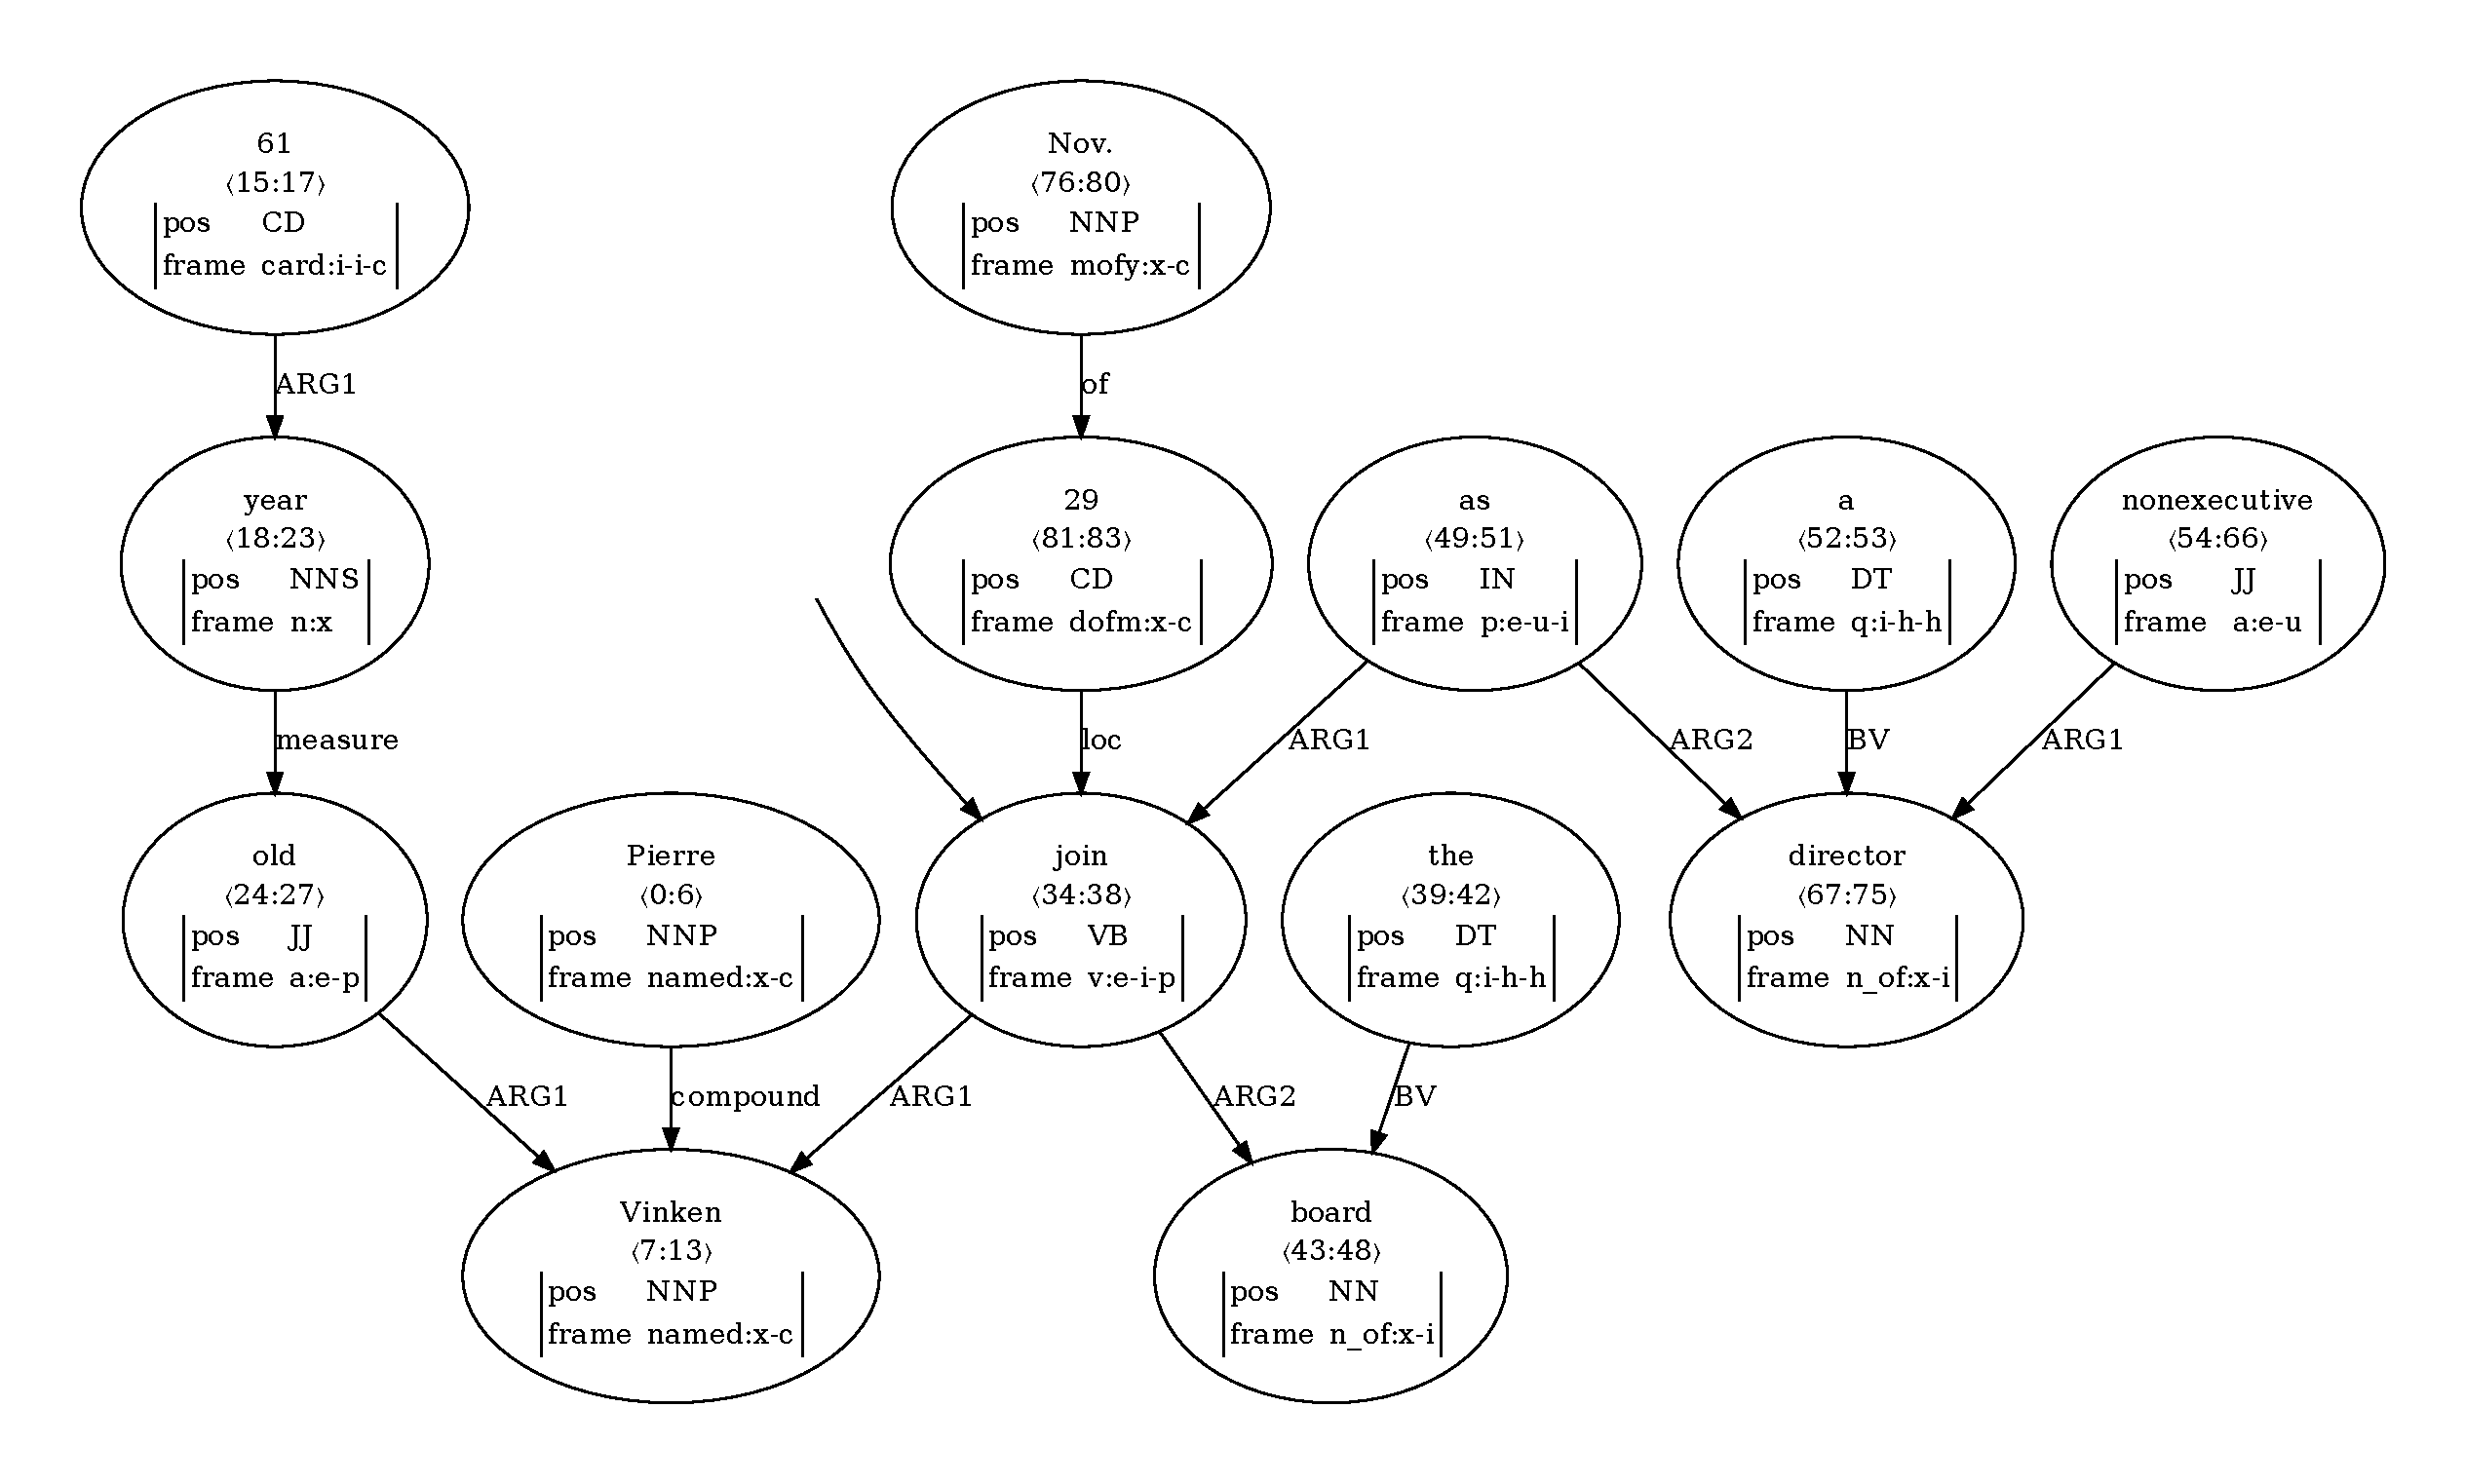
\includegraphics[width=0.90\textwidth]{bg/dm-20001001.pdf}
\caption{\label{fig:bg-dm}The DM representation for the sentence
  \#20001001}
\end{figure}

\Paragraph{DM: DELPH-IN MRS-Derived Bi-Lexical Dependencies} It
originates in a manual re-annotation, dubbed
DeepBank~\citep{Fli:Kor:Zha:12}, with syntactico-semantic analyses of
the LinGO English Resource Grammar~\citep{Oep:Fli:Tou:04} in logical
forms. These logical forms are often referred to as English Resrouce
Semantics~\citep[ERS,][]{Ben:Fli:Oep:15}, and the underlying grammar
is rooted in the general linguistic theory of Head-Driven Phrase
Structure Grammar~\citep[HPSG,][]{Pol:Sag:94}.

Then \citet{Iva:Oep:Ovr:12} propose a two-stage version to transform
the ERS logical forms into bi-lexical semantic dependency graphs. As
shown in the~\autoref{fig:dm-psd-history}, ERS logical forms are
firstly tranformed into Elementary Dependency
Structures~\cite[EDS,][]{Oep:Lon:06}, then EDS are simplified into
pure bi-lexical dependencies, dubbed DELPH-IN MRS Bi-Lexical
Dependencies~(or DM). As shown in~\autoref{fig:bg-dm}, graph nodes in
DM are anchoring to the surface tokens. Hence, DM is
lexical-anchoring. However, the underlying sentence is not fully
covered in the graph. For example, the word ``will" does not produce
any node in the DM graph. Edges mainly indicate semantic argument
roles~(ARG1, ARG2, ...) into the relation corresponding to their
source node~\footnote{The annotation of predicate-arugment structures
  is based on the semantic inferface~(SEM-I) in the ERG. Please refer
  to this introduction for more
  details.\url{https://github.com/delph-in/docs/wiki/ErgSemantics_Interface}},
but there are some more specialized edge labels too. For example, it
uses \kw{compound} to reflect the name ``Pierre Vinken" as a whole,
and uses BV (bound variable, e.g., the word 'a') as a reflection of
quantification in the underlying logic quantification. \textit{In a sum, DM is
lexical-anchoring, and it captures semantic phenomena including
predicate-argument structures, word-sense differentiation,
quanitification and scope.}

\begin{figure}[!th]
\centering
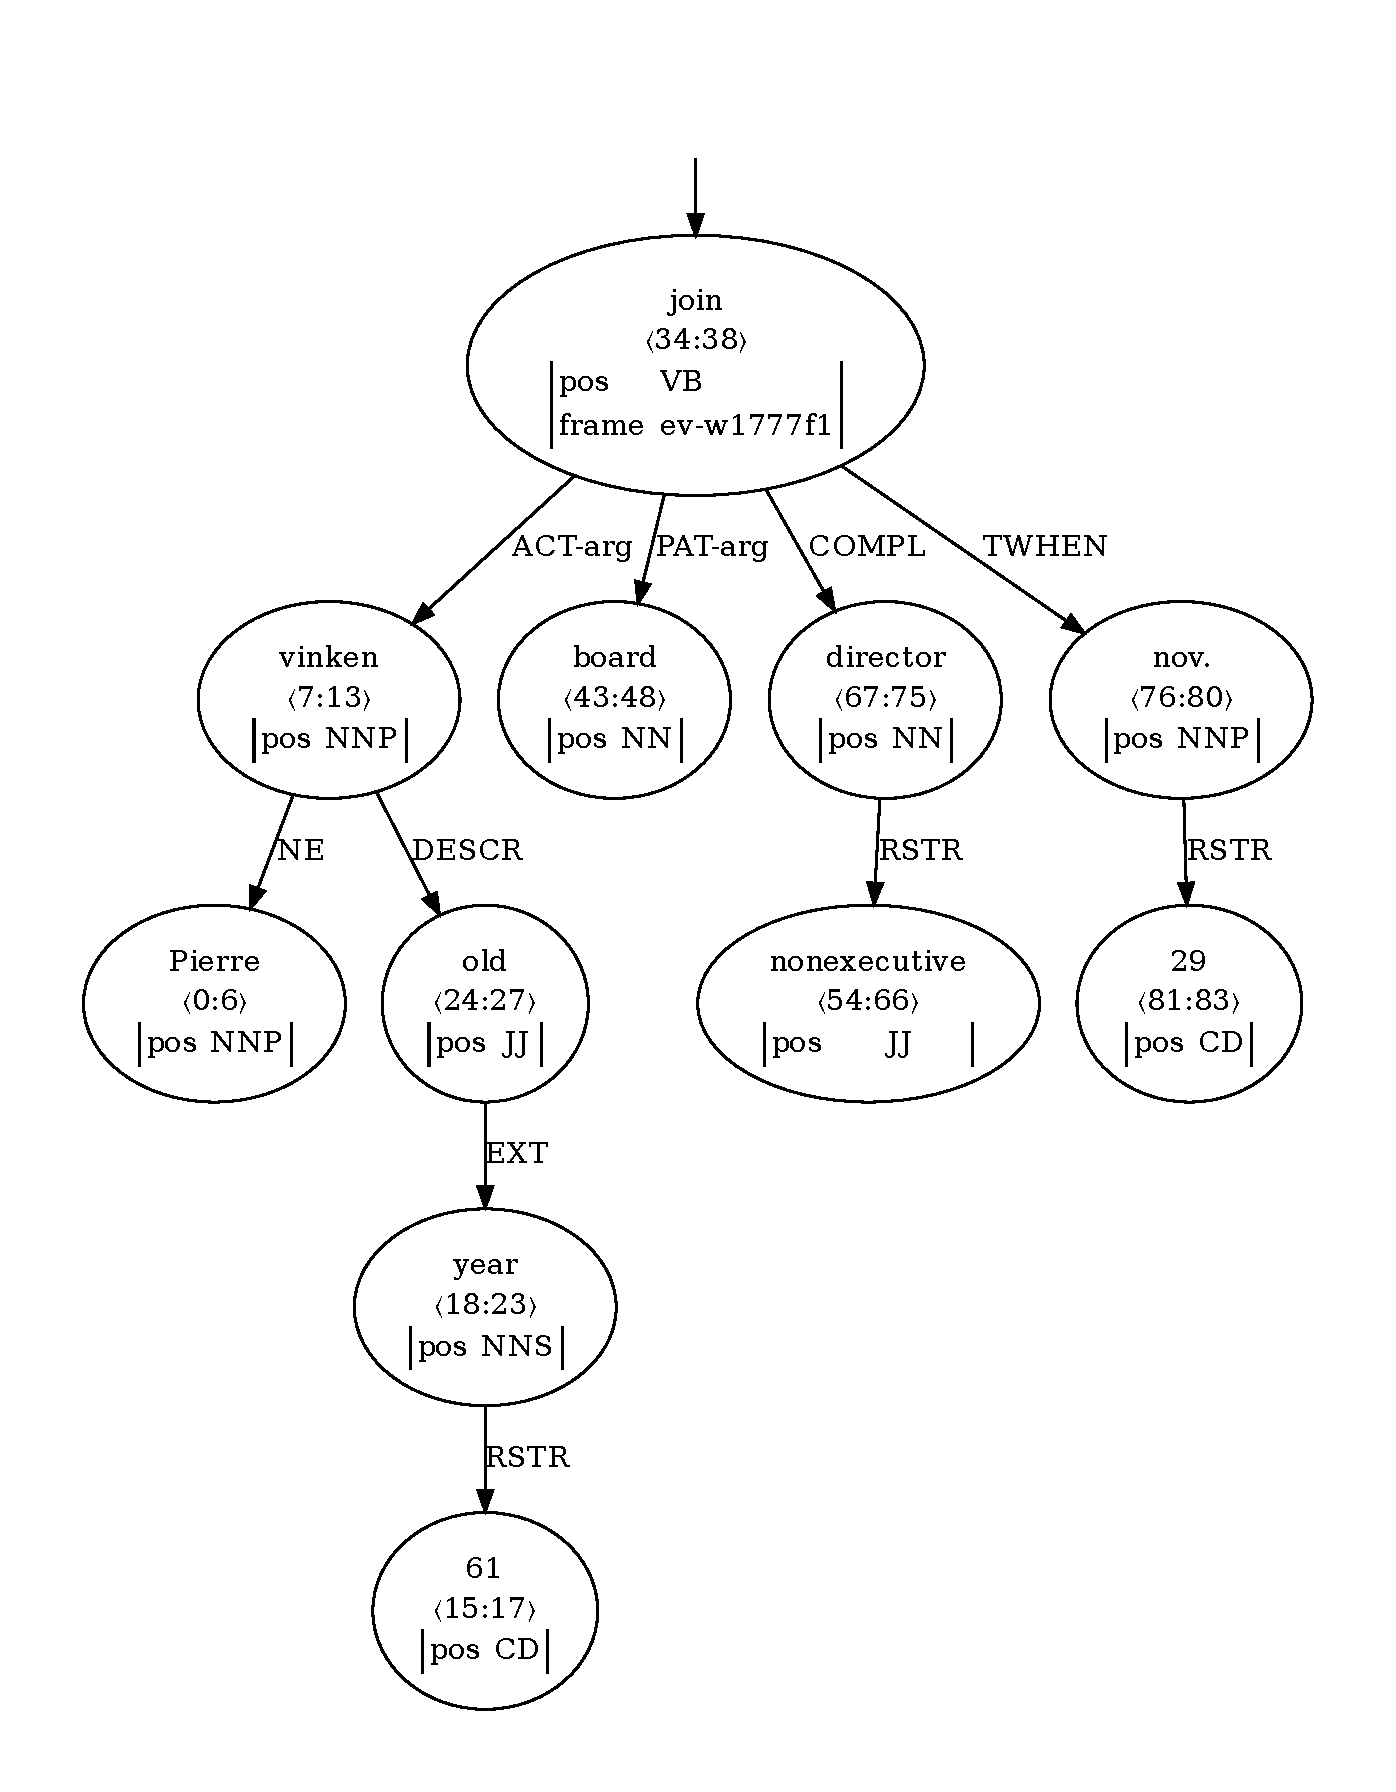
\includegraphics[width=0.98\textwidth]{bg/psd-20001001.pdf}
\caption{\label{fig:bg-psd}The PSD representation for the sentence
  \#20001001}
\end{figure}


\Paragraph{Prague Semantic Dependencies} Besides DM, there is another
line of research to simplify the richer syntacticosemantic
representations into bi-lexical semantic dependencies.  It adopts the
reduction of tectogrammatical trees (or t-trees) from the linguistic
school of Functional Generative
Description~\citep[FGD,][]{Sga:Haj:Pan:86,hajic2012announcing} into
PSD. The Prague Czech-English Dependency
Treebank~\citep[PCEDT,][]{hajic2012announcing} is a set of parallel
dependency trees over the WSJ texts from the PTB, and their Czech
translations. The PSD bi-lexical dependencies are extracted from the
tectogrammatical annotation layer. Top nodes are derived from t-tree
roots; Especially, they mostly correspond to main verbs. In case of
coordinate clauses, there are multiple top nodes per
sentence. \autoref{fig:bg-psd} shows the PSD represention of our
example sentence. One major difference are the role labels and verb
frames, they are grounded in a machine-readable valency
lexicon~\citep{urevsova2016czengvallex}, and the frame values on
verbal nodes indicate specific verbal senses in the lexicon. \textit{In a
summary, PSD is also lexical-anchoring, and it captures the same
sementic contents with DM~(inclduing predicate-argument structures,
word-sense, quatification and scope), however, with the different
formation and different frame lexicon.}

\begin{figure}[!th]
  \centering
  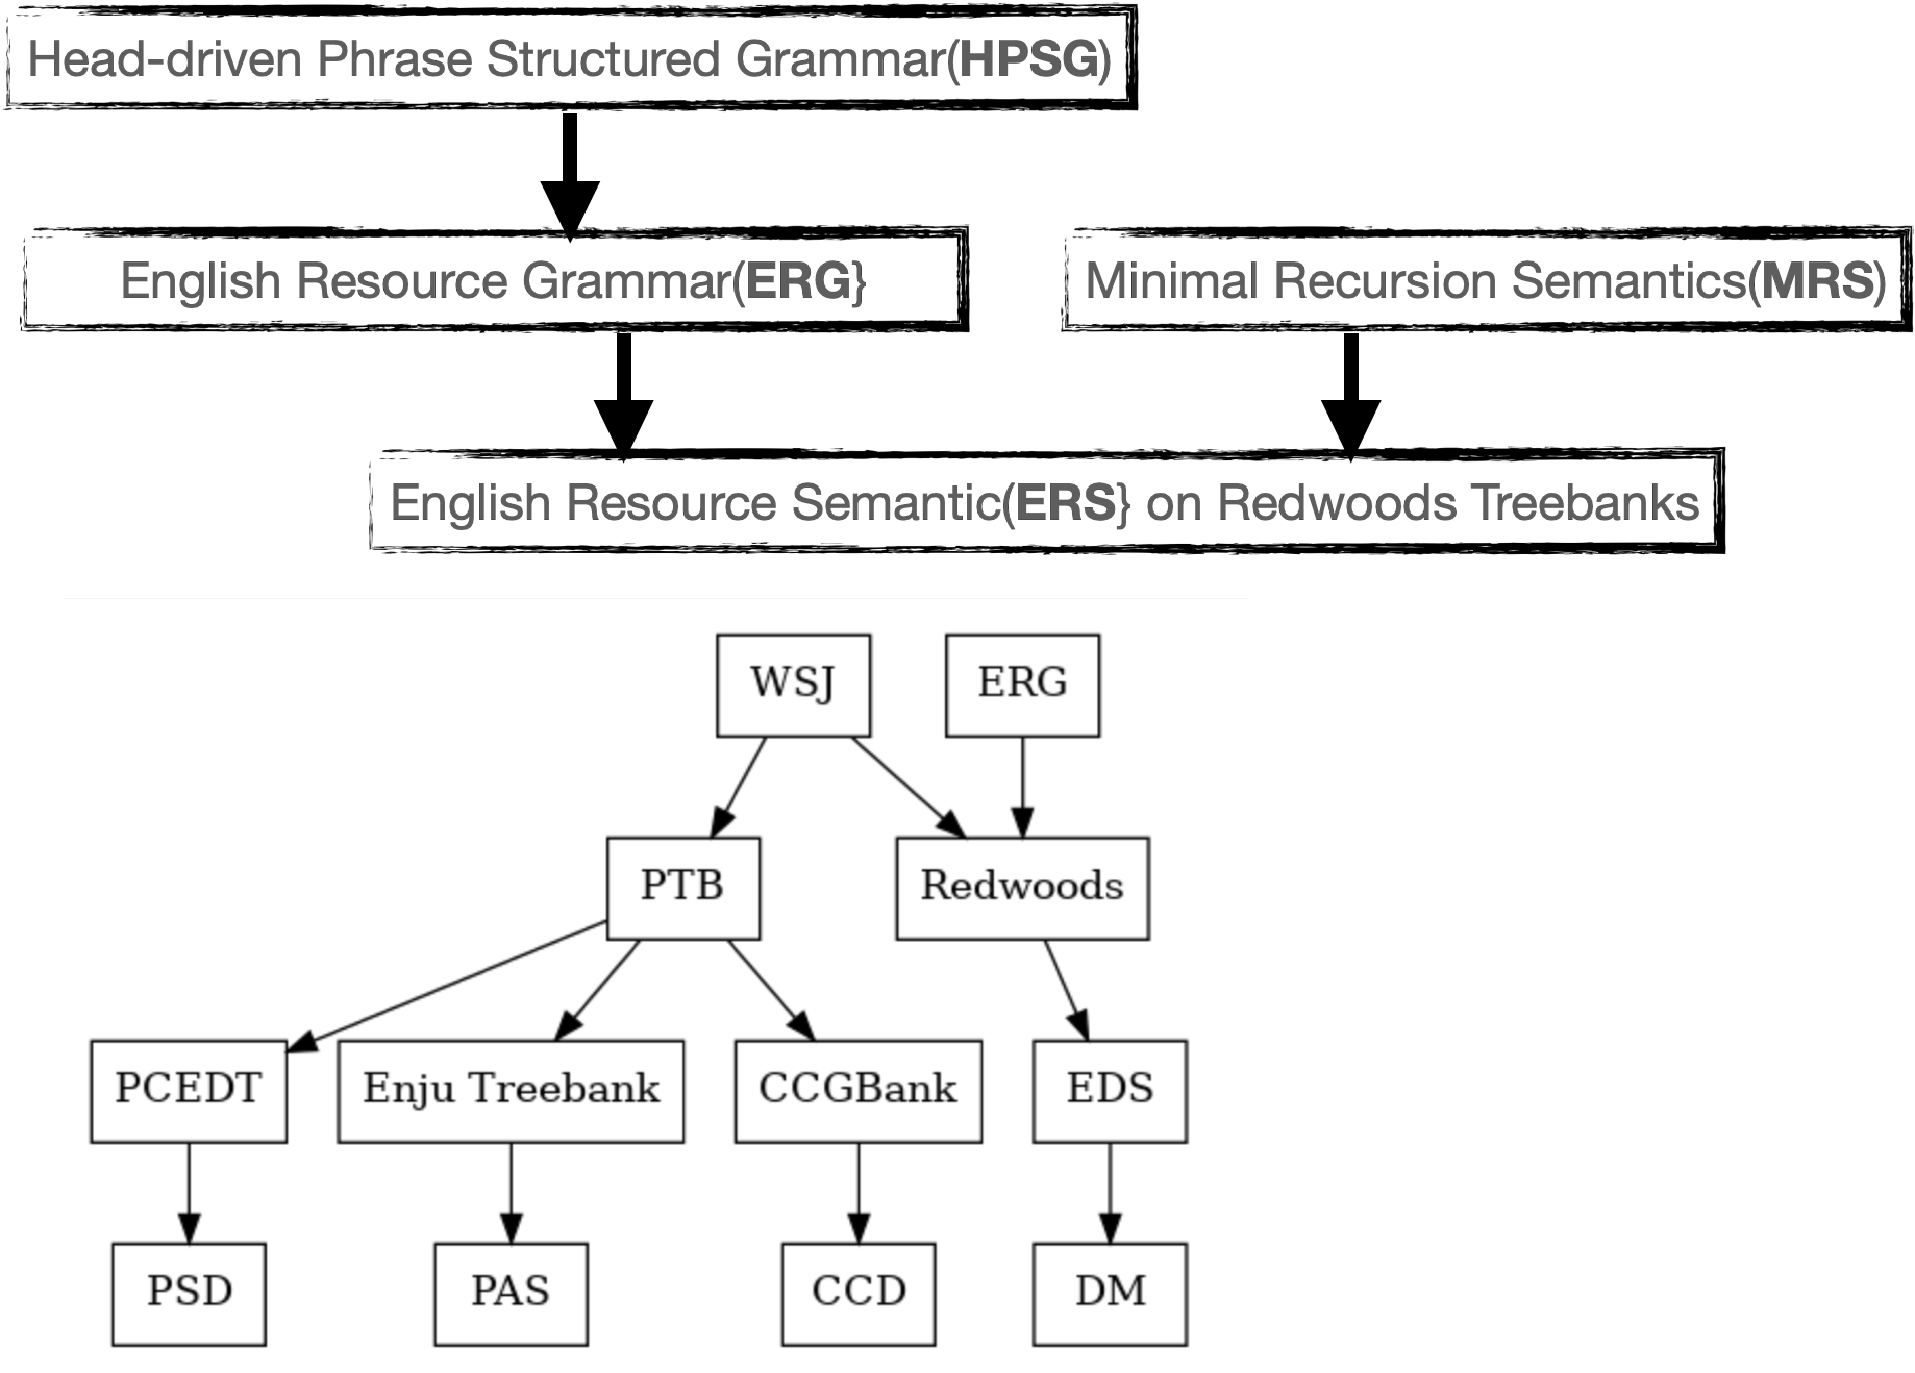
\includegraphics[width=0.98\textwidth]{bg/dm-psd-history.pdf}
\caption{\label{fig:dm-psd-history}The hierarchical relations between
  DM, PSD, and their underlying grammar and semantics}
\end{figure}


\subsubsection{Abstract Meaning Representation}
\label{ssec:bg:amr}
%
\begin{figure}[!th]
\centering
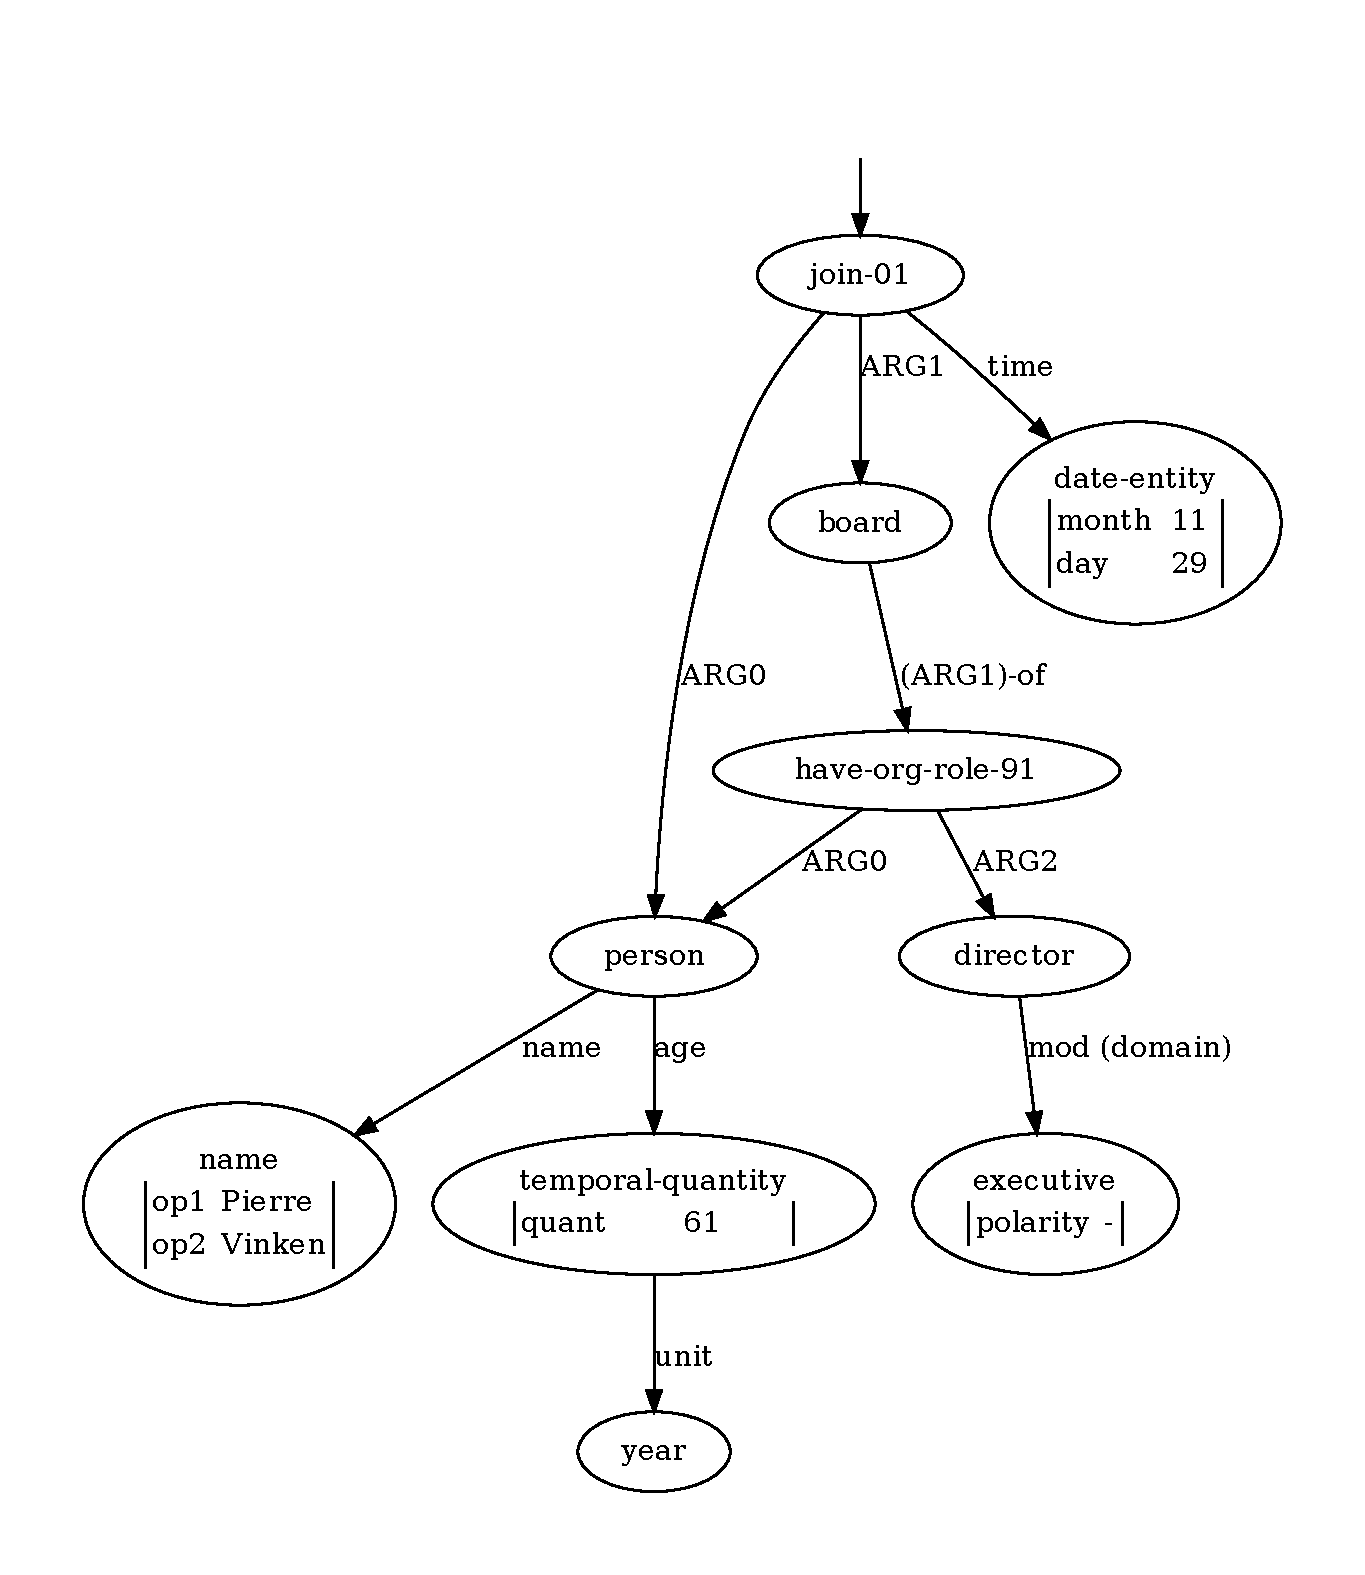
\includegraphics[width=0.98\textwidth]{bg/amr-20001001.pdf}
\caption{\label{fig:bg-amr} The AMR representation for the sentence
  \#20001001}
\end{figure}

As shown in~\autoref{fig:bg-amr}, Abstract Meaning Representation
represents sentence meaning as directed graphs with labeled nodes
~(concepts) and edges~(relations). AMRs are rooted, labeled graphs
that are easy for people to read, and easy for programs to traverse.
AMR concepts are either English words (``board"), PropBank framesets
(``join-01"), or special entity keywords~(``date-entity", ``person",
``name", etc.), quantities~(``temporal-quantity",
``distance-quantity", etc.), and logical conjunctions~(``and", etc).
AMR strives for a more logical, less syntactic representation.  For
example, it represent the word ``nonexecutive" with a negation
``(:polarity 0)" with the concept ``executive". Further more,
different from DM and PSD on predicate-argument representation, AMR
makes extensive use of PropBank framesets~\citep{Kin:Pal:02,
  palmer2005proposition}. For example, It represents the verb ``join"
using the frame “join-01”. At the mean time, AMR also newly designs
special frames to reuse those core roles in Propbank. As shown in
~\autoref{fig:bg-amr}, the word ``board" have a role ``ARG1-of" to a
special frame ``have-org-role-91".

The above abstraction allows for concepts and relations not explicitly
mentioned in the text, but leaves open the question of how these are
derived from the text. This question is important because training
statistical AMR parsers typically starts with a conjectured alignment
between tokens and the graph elements. Most AMR
parsers~\cite[\eg][]{Flanigan:2014vc,Wang:2015uo,Artzi:2009tb,Pust:2015ug,Peng:2015tj,Konstas:2017uj,Wang:2017vt}
use either the JAMR aligner~\cite{Flanigan:2014vc} or the ISI
aligner~\cite{Pourdamghani:2014aligning} for this
purpose\footnote{Other aligners exist -- \eg,
  \citet{chen2017unsupervised} uses dependencies, but raw text
  alignments are more prevalent.}  We introduced more details about
AMR alignment in ~\autoref{sssec:lex-phr:amr-anchor}, and we show that
AMR nodes and subgraphs are actually implicitly anchored to the
lexical tokens or entities. \textit{In a sum, AMR is implicit
  lexical-anchorin, and it captures more semantic content than DM and
  PSD. Besides the common predicate-argument structure, word sense,
  qutification, scope~(by placing `polarity'), AMR also represents the
  lexical decomposion, anaphoric coreference and entity-linking.}


\subsubsection{Universal Conceptual Cognitive Anotation}
\label{ssec:bg:ucca}

\begin{figure}[!th]
\centering
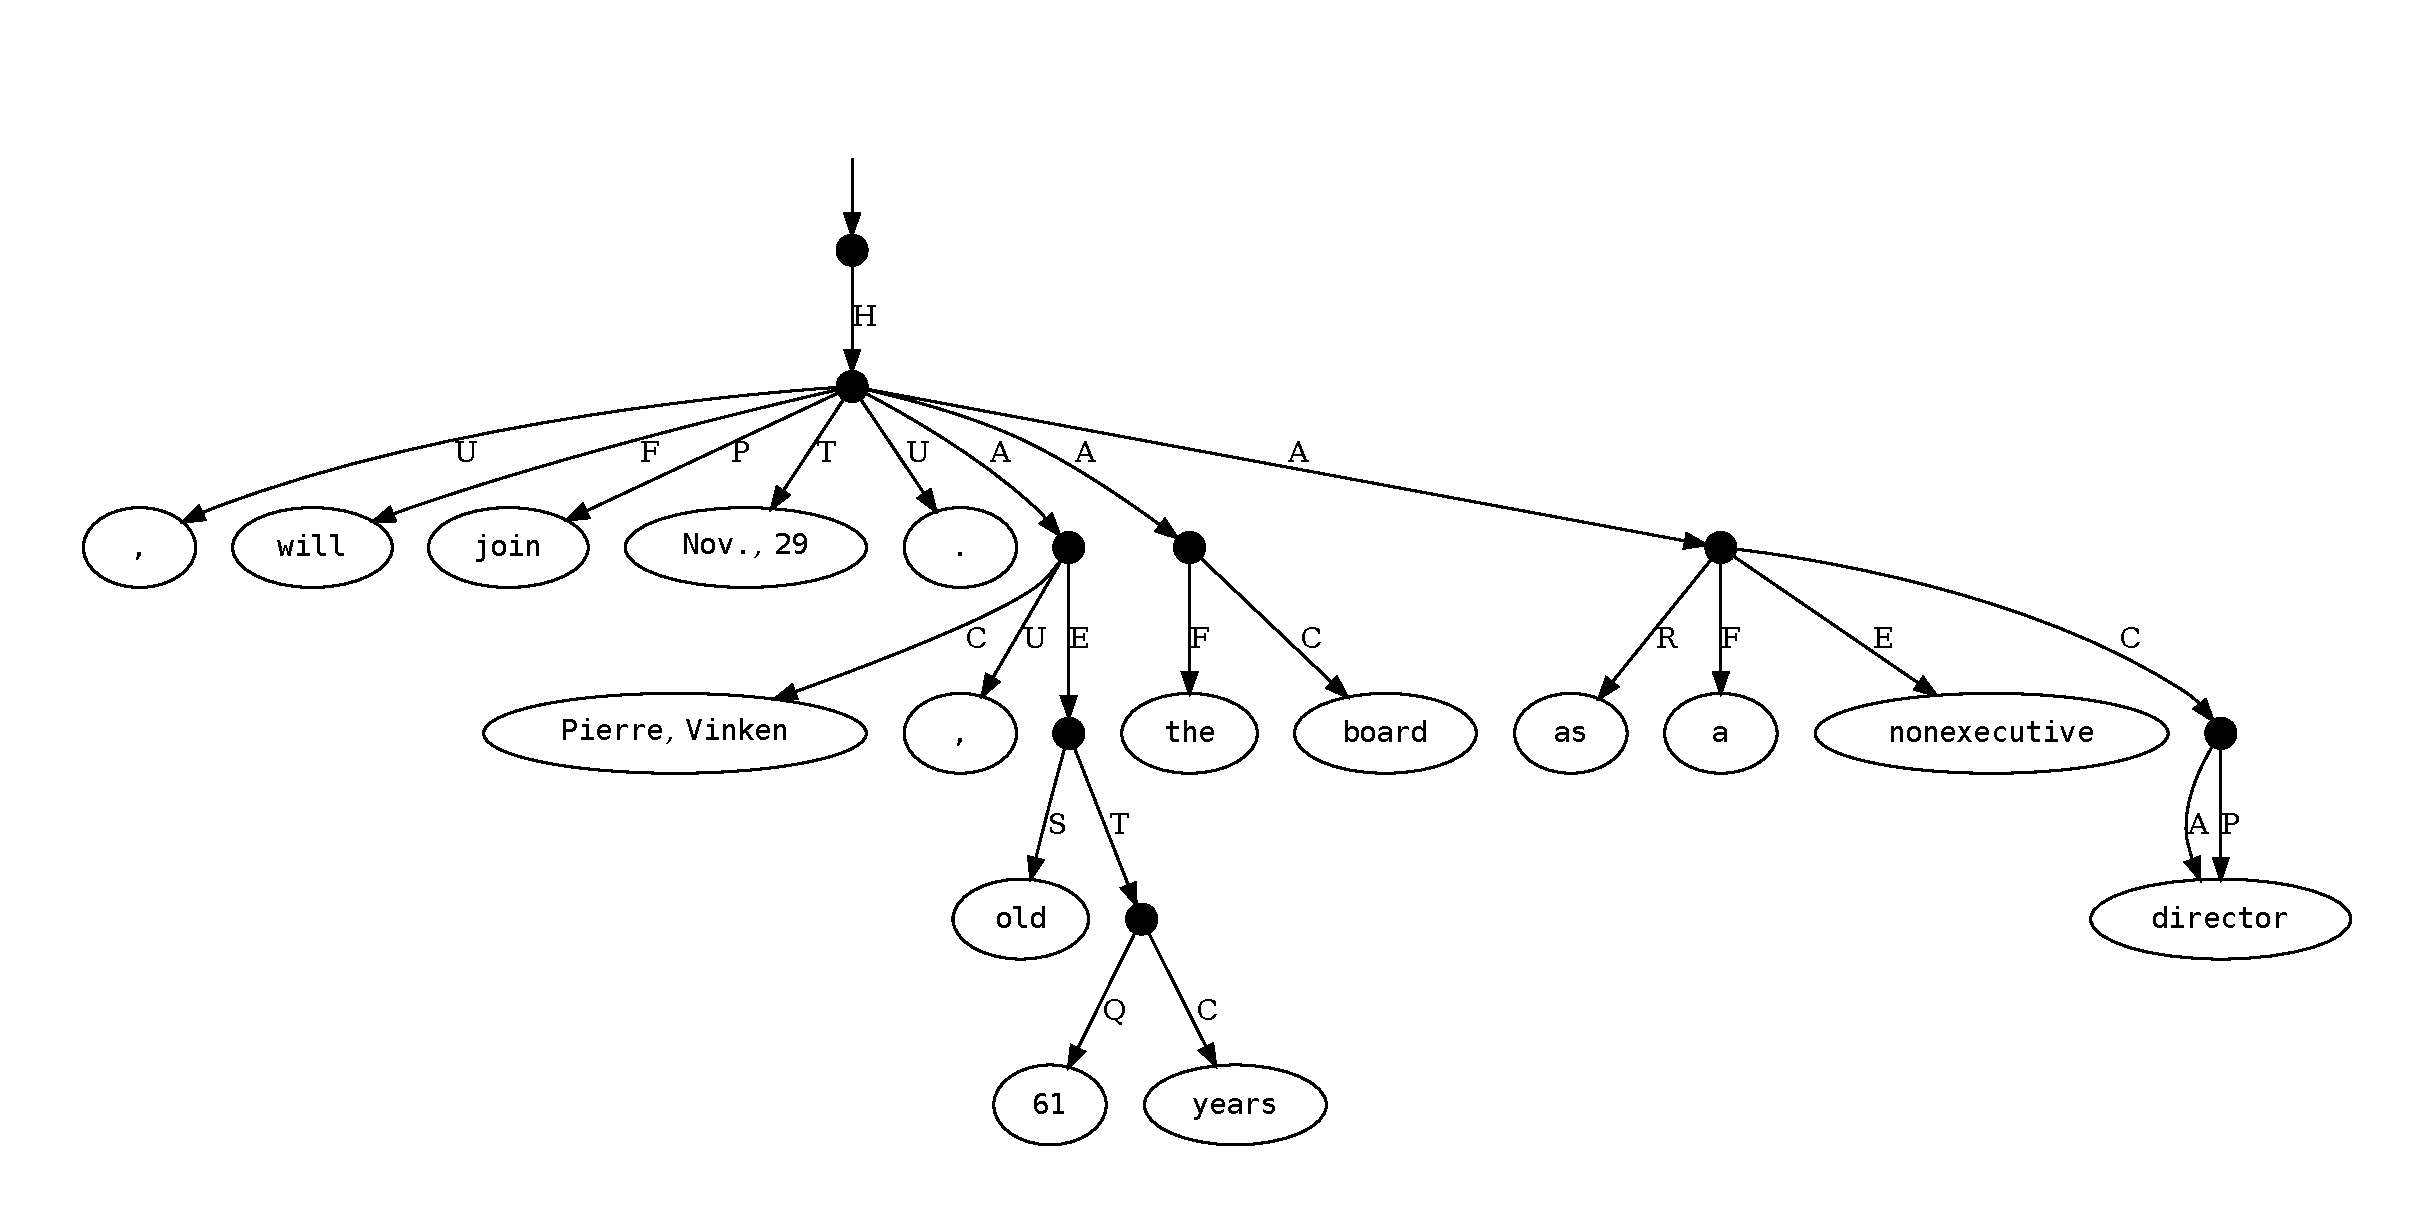
\includegraphics[width=0.98\textwidth]{bg/ucca-20001001.pdf}
\caption{\label{fig:bg-ucca}The UCCA representation for the sentence
  \#20001001}
\end{figure}

Similar with AMR, UCCA is designed to abstract the semantic scheme
away from its surface from and syntactic forms. UCCA uses directed
acyclic graphs (DAGs) to represent its semantic structures. The atomic
meaning-bearing units are placed at the leaves of the DAG and are
called terminals. The nodes of the graph are called units. A unit may
be either (i) a terminal or (ii) several elements jointly viewed as a
single entity according to some semantic or cognitive
consideration. In many cases, a non-terminal unit is comprised of a
single relation and the units it applies to (its arguments), although
in some cases it may also contain secondary relations. Hierarchy is
formed by using units as arguments or relations in other units.

While different from previous DM, PSD and AMR, categories are not
annotated on nodes, but on edges and represent the descendant unit's
role in forming the semantics of the parent unit. The foundational
layer is designed to cover the entire text, so that each word
participates in at least one unit. It focuses on argument structures
of verbal, nominal and adjectival predicates and the inter-relations
between them. Argument structure phenomena are considered basic by
many approaches to semantic and grammatical representation, and have a
high applicative value, as demonstrated by their extensive use in
NLP. The foundational layer views the text as a collection of
Scenes. A Scene can describe some movement or action, or a temporally
persistent state. As shown in~\autoref{fig:bg-ucca}, for the event
`join the board', `join' with an incoming edge `P' denoting the
category ``Process", which is the main relation of a scene that
evolves in time. While the edge `A' linked to the non-terminal node
corresponding to ``Pierre, Vinken, 61 years old" means the unit
``Pierre, Vinken" is the participant of the scene. In a sum, UCCA is
phrasal-anchoring, and its foundational layer captures
predicate-argument structures, anaphoric coreference, representing
less semantic content than DM,PSD, and AMR. However, UCCA shows more
benefits on cross-ligual, easy annotation and extensible modualrity.


\subsubsection{Summary of Broad-Coverage Meaning Representation}
\label{ssec:bg:summary-broad-coverage}
For easy reference, in~\autoref{tbl:summary-broad-coverage}, we summerize the background of
broad-coverage meaning representations with respect to the their
anchoring type and captured semantic phenomena. For more detailed
comparative studies over the state-of-art semantic representation,
please refer to the paper~\cite{abend2017state}.

\begin{table}[ht]
  \begin{center}
\setlength{\tabcolsep}{4pt}
{\small
\begin{tabular}{c|cccc}
\toprule
\hline
                        & DM               & PSD              & AMR              & UCCA    \\ \hline
Anchoring Type          & Explicit Lexical & Explicit Lexical & Implicit Lexical & Phrasal \\ \hline
Predicate-Argument      & Yes              & Yes              & Yes              & Yes     \\
Word Sense              & Yes              & Yes              & Yes              & No      \\
Qualification and Scope & Partial          & No               & Yes              & No      \\
Presupposition/Focus    & No               & No               & Yes              & No      \\
Lexical Decomposition   & No               & No               & Yes              & No      \\
Anaphoric Coreference   & No               & No               & Partial          & Partial \\
Grounding               & No               & No               & Yes              & No \\ \hline
\bottomrule

\end{tabular}}
\end{center}
\caption{The summary of broad-coverage meaning representation, with respect to their anchoring type and captured semantic contents}
\label{tbl:summary-broad-coverage}
\end{table}


\subsection{Application-specific Representation on Dialogue}
\label{ssec:bg:dialogue-mr}

In this thesis, we ground the study on application-specific
representation on dialogue. The following section will introduce the
dialog rerepsentations via dialogue act, dialog state and richer
conversational semantic representations.

\subsubsection{Dialogue Act and MISC Codes}
\label{sssec:bg:dialogue-act}
In utterance-level, dialogue acts are designed to represent the
function of each utterance in the dialogue. The key insight behind
dialgue act is that each utterance in a dialogue is a kind of action
being performed by the speaker. The history of dialogue act can be
derived back to the philosopher~\citet{wittgenstein2010philosophical}.
A dialogue act has two main components: a communicative function and a
semantic content. \citet{bunt2010towards} provides an ISO project
developing an international standard for annotating dialogue with
semantic information, in particular concerning the communicative
functions of the utterances, the kind of content they address, and the
dependency relations to what was said and done earlier in the
dialogue. Similarly, Motivational Interview Skill Codes
~\cite[MISC,][]{miller2003motivational,miller2012motivational} are
also proposed to represent the functions of each client and therapist
utterance in the psychotherapy dialogue. In this part, we will mainly
introduce the MISC Codes for psychotherapy dialogue.

%% putting the table here to make it in the second page.
\begin{table}[ht]
  \begin{center}
\setlength{\tabcolsep}{4pt}
{\small
\begin{tabular}{llll}
  \toprule
  {\bf Code}            & {\bf Count}            & {\bf Description}                                                                                            & {\bf Examples}                                    \\
  \midrule \midrule
  \multicolumn{4}{c}{ \bf Client Behavioral Codes }                                                                                                                                                                 \\
  \midrule
  \multirow{2}{*}{\FN}  & \multirow{2}{*}{47715} & \multirow{2}{*}{\parbox{5.5cm}{Follow/ Neutral: unrelated to changing or sustaining behavior.}}              & ``You know, I didn't smoke for a while.''         \\
                        &                        &                                                                                                              & ``I have smoked for forty years now.''            \\
  \CHANGE               & \multirow{2}{*}{5099}  & \multirow{2}{*}{\parbox{5.5cm}{Utterances about changing unhealthy  behavior.}}                                                                          & ``I want to stop smoking.''                       \\
                        & \\
  \SUSTAIN              & \multirow{2}{*}{4378}  & \multirow{2}{*}{\parbox{5.5cm}{Utterances about sustaining unhealthy behavior.}}                                                                        & ``I really don't think I smoke too much.''        \\
                        & \\ \midrule
  \midrule
  \multicolumn{4}{c}{\bf Therapist Behavioral Codes }                                                                                                                                                               \\
  \midrule
  \FA                   & 17468                  & Facilitate conversation                                                                                      & ``Mm Hmm.'', ``OK.'',``Tell me more.''            \\
  \GI                   & 15271                  & Give information or feedback.                                                                                & ``I'm Steve.'', ``Yes, alcohol is a depressant.'' \\
  \multirow{2}{*}{\RES} & \multirow{2}{*}{6246}  & \multirow{2}{*}{\parbox{5.5cm}{Simple reflection about the client's most recent utterance.}}                 & C: ``I didn't smoke last week''                   \\
                        &                        &                                                                                                              & T: ``Cool, you avoided smoking last week.''       \\
  \multirow{2}{*}{\REC} & \multirow{2}{*}{4651}  & \multirow{2}{*}{\parbox{5.5cm}{Complex reflection based on a client's conversation history.}} & C: ``I didn't smoke last week.''                  \\
                        &                        &                                                                                                              & T: ``You mean things begin to change''.           \\
  \QUC                  & 5218                   & Closed question                                                                                              & ``Did you smoke this week?''                      \\
  \QUO                  & 4509                   & Open question                                                                                                & ``Tell me more about your week.''                 \\
  \multirow{2}{*}{\MIA} & \multirow{2}{*}{3869}  & \multirow{2}{*}{\parbox{5.5cm}{MI adherent,~\eg, affirmation, advising with permission, etc.}}          & ``You've accomplished a difficult task.''         \\
                        &                        &                                                                                                              & ``Is it OK if I suggested something?''            \\
  \multirow{2}{*}{\MIN} & \multirow{2}{*}{1019}  & \multirow{2}{*}{\parbox{5.5cm}{MI non-adherent,~\eg, confront, advising without permission, etc.}}      & ``You hurt the baby's health for cigarettes?''    \\
                        &                        &                                                                                                              & ``You ask them not to drink at your house.''      \\\bottomrule
\end{tabular}}
\end{center}
\caption{Distribution, description and examples of MISC labels.}
\label{tbl:misc}
\end{table}

Motivational Interviewing~(MI) is a style of psychotherapy that seeks
to resolve a client's ambivalence towards their problems, thereby
motivating behavior change. Several meta-analyses and empirical
studies have shown the high efficacy and success of MI in
psychotherapy~\citep{burke2004emerging, martins2009review,
  lundahl2010meta}. However, MI skills take practice to master and
require ongoing coaching and feedback to sustain~\citep{Schwalbe2014}.
Given the emphasis on using specific types of linguistic behaviors in
MI~(\eg, open questions and reflections), fine-grained behavioral
coding plays an important role in MI theory and training.

Motivational Interviewing Skill Codes~(MISC, ~\autoref{tbl:misc}) is a
framework for coding MI sessions. It facilitates evaluating therapy
sessions via utterance-level labels that are akin to dialogue
acts~\citep{stolcke2000dialogue,jurafsky2018speech}, and are designed
to examine therapist and client behavior in a therapy
session.\footnote{The original MISC description of
  \citet{miller2003manual} included 28 labels (9 client, 19
  therapist). Due to data scarcity and label confusion, various
  strategies are proposed to merge the labels into a coarser set.  We
  adopt the grouping proposed by~\citet{xiao2016behavioral}; the
  appendix~\autoref{sec:misc_clustering} gives more details.}
\autoref{tbl:misc} shows the distritbution, description and examples
of MISC labels for clients and therapist. Each of the MISC label will
be corresponding to the a single utterance. \textit{Hence, MISC code
prediction is a sentence-anchoring task, and it mainly captures the
function of each utterance.}

\subsubsection{Dialog State Tracking}
\label{ssec:bg:dialogue-state}

\begin{figure}[!ht]
\centering
  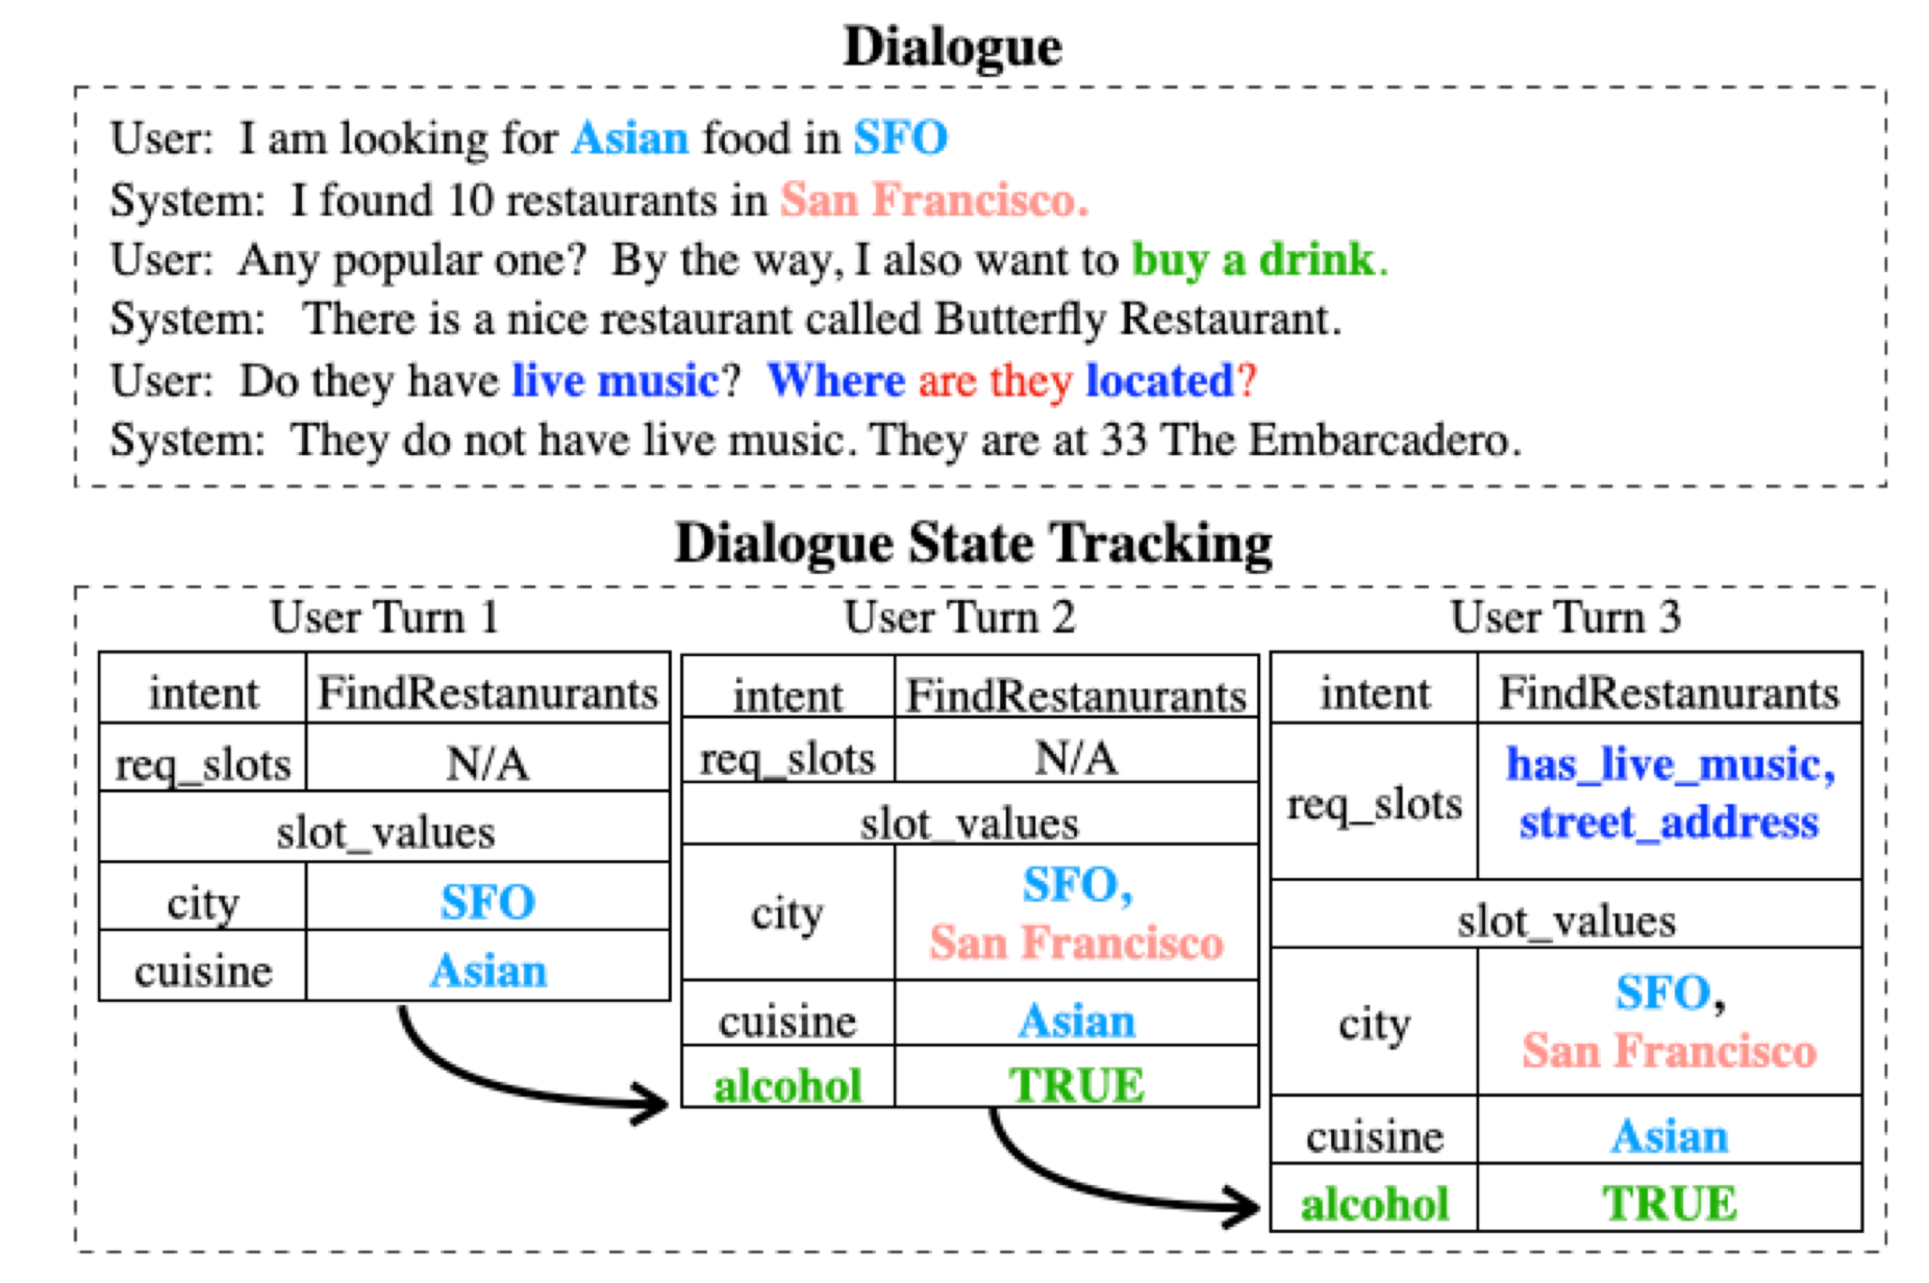
\includegraphics[width=0.90\textwidth]{dst.pdf}
  \caption{\label{fig:dst} An example dialogue, along with its dialog state representation for  the intent, requested slot, slot values}
\end{figure}

From the simple GUS~\citep{bobrow1977gus} to the modern task-based
dialogue systems built in virtual assistants~(Alexa, Siri, and Google
Assistant~\etal), they are all based around frames. Frame theory is
derived from Fillmore's case theory~\citep{Fillmore:68}. A frame is a
kind of knowledge structure representing the kinds of intentions the
system can extract from user sentences, and consists of a collection
of slots, each of which can take a set of possible values. Together
this set of frames is sometimes called a domain ontology.

As the dialogue goes on, a dialogue state tracker maintains the
current state of the dialogue (which include the user's most recent
dialogue intent, plus the entire set of slot-filler constraints the
user has expressed so far). The dialogue policy decides what the
system should do or say next. Finally, dialogue state systems have a
natural language generation component to reply the utterance to users.

\autoref{fig:dst} shows a dialogue on restaurant booking service. For
each user turn, the dialogue state tracking is to predict the
corresponding intent, requested slot, slot values for that turn. The
intent classification task is to understand what the user trying to
accomplish in this dialogue utterance, thus the output intent label is
anchored to the current user utterance. The requested slot is what the
user is asking for more information, while the slot filling task is to
extract the particular slots and fillers that the user offered to the
system for more detailed arguments of their intent. The requested
slots aand slot-filling tasks can depend on any relevant tokens or
phrases in the user utterance, thus the anchoring is mixed anchoring.

\subsubsection{Conversational Semantic Representation}
\label{ssec:bg:dialogue-rep}
Most existing annotations for task oriented dialog systems have fallen
on the extremes of non-recursive intent and slot tagging, such as in
the MultiWOZ~\cite{budzianowski2018multiwoz}. Hence, the previous
intent-slot dialog state representation have poor compositionality to
represent complex conversational request, such multiple intents in the
same utterance, and nested intent slot structures.
\begin{figure}[!th]
\centering
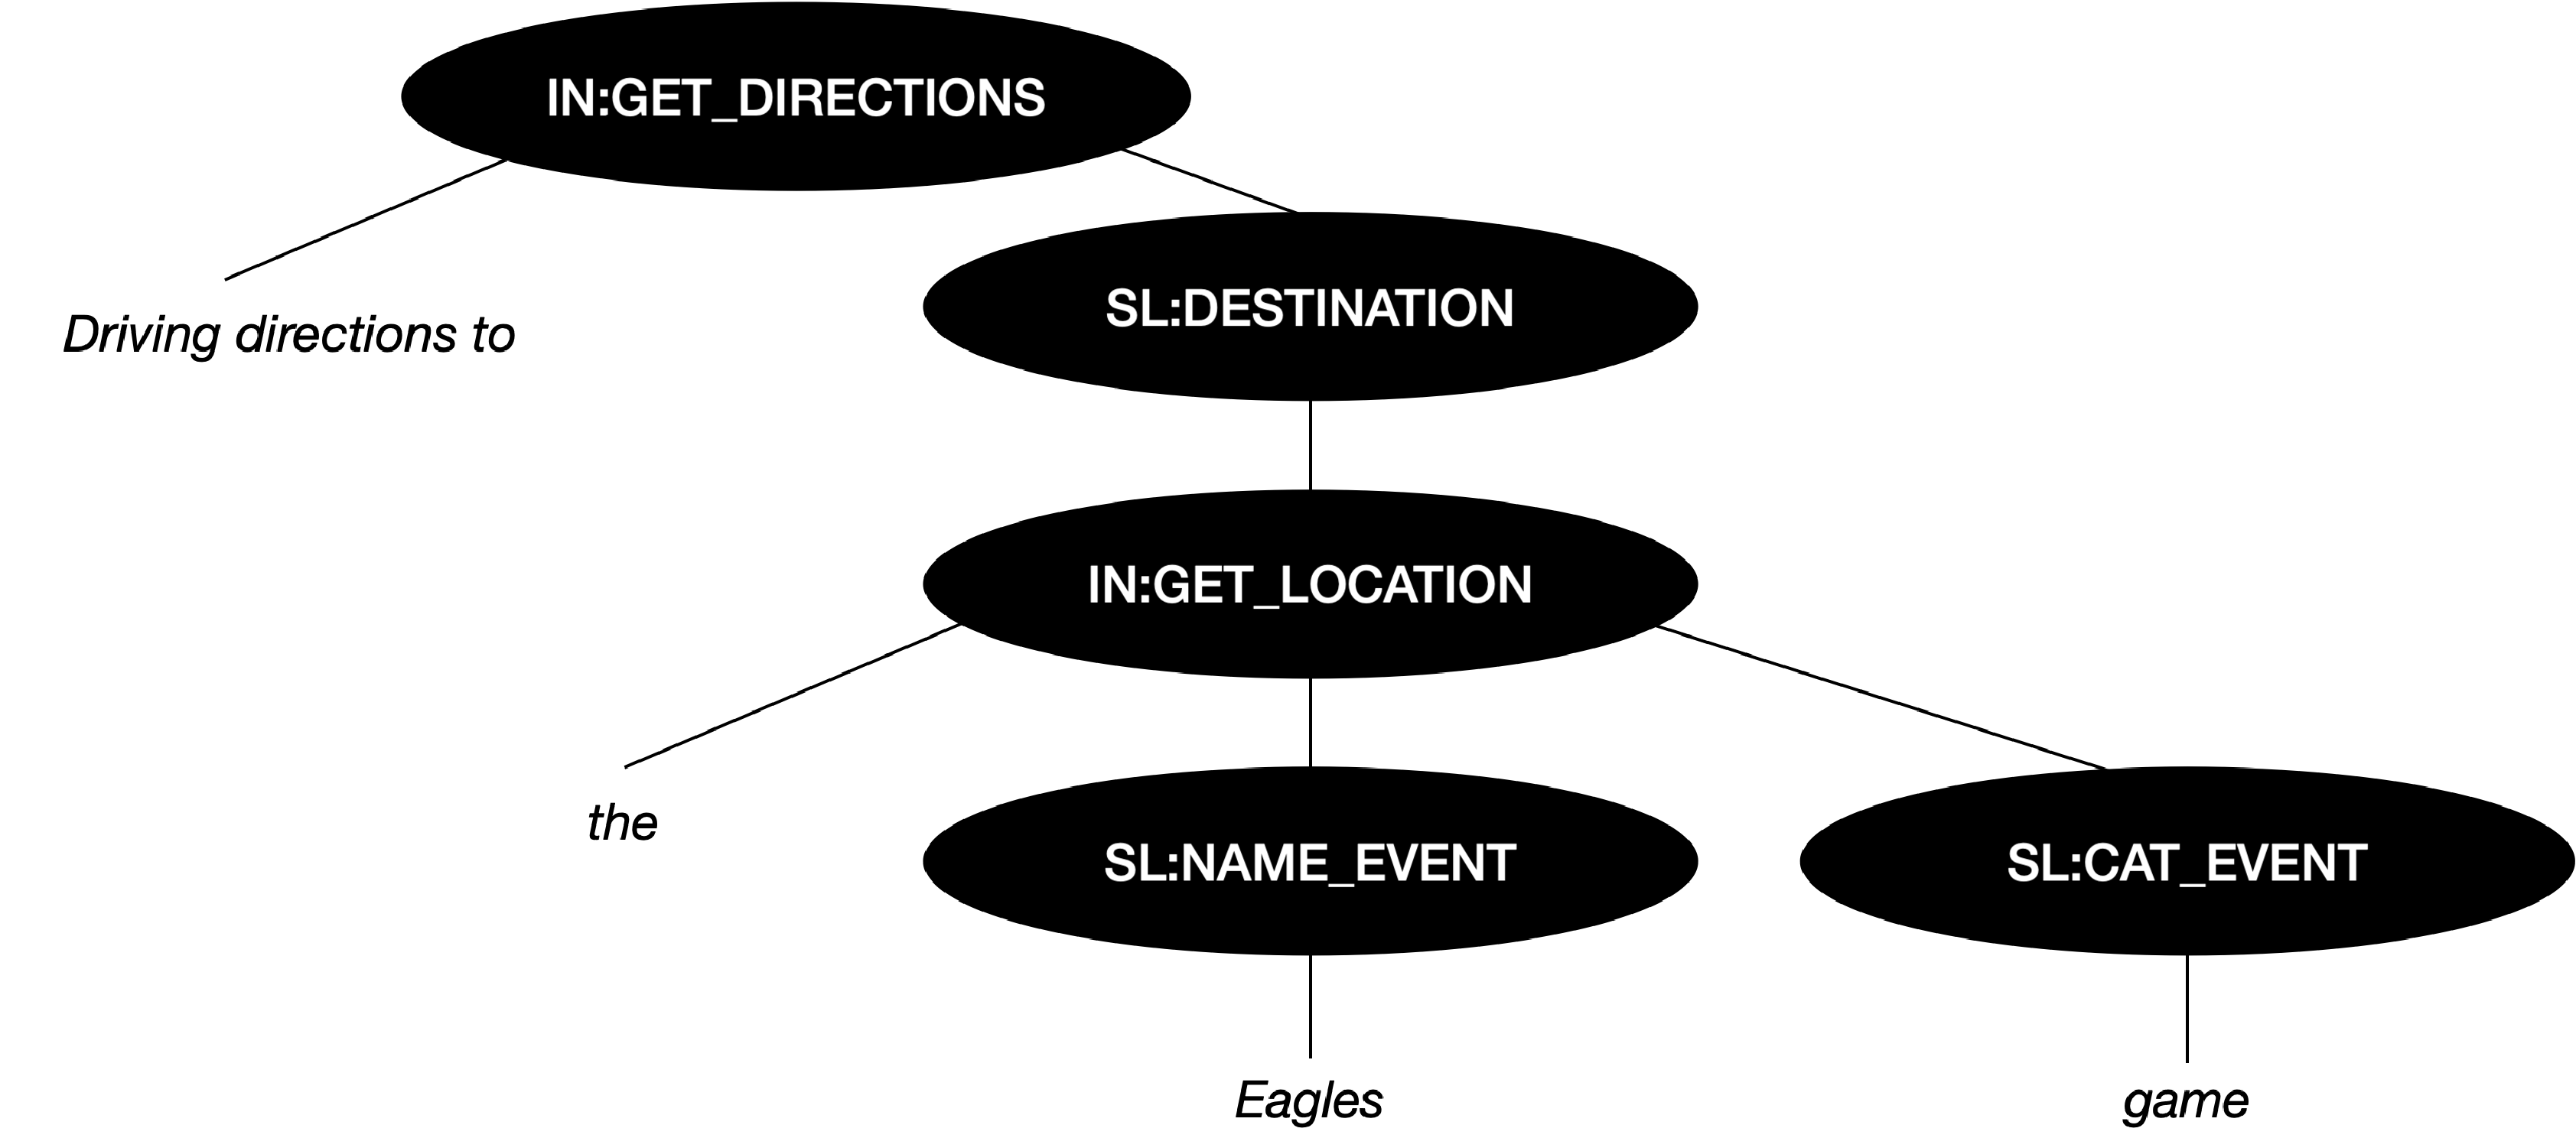
\includegraphics[width=0.95\textwidth]{top-driving.pdf}
\caption{\label{fig:top-example} TOP examples for conversational
  semantic parsing~(borrowed from the original
  paper~\citep{gupta-etal-2018-semantic-parsing})}
\end{figure}

Recently, conversational parsing has attract much attention to
represent the dialogue state in a more compositional way, such as the
hierarchical tree structure in the Task-Oriented dialogue Parsing
~\cite[TOP,][]{gupta-etal-2018-semantic-parsing,aghajanyan2020conversational},
~\cite[TreeDST,][]{cheng2020conversational}, and
~\cite[Dataflow,][]{andreas2020task}. In a summ, those conversation
semantic representation offers richer intent slot compositions, and
support complex conversational linguistic phenomenos, such as dialogue
state revision and recovering.

In this thesis, we study the structures of single sentence
representation TOP for dialogue
representations. \autoref{fig:top-example} shows two examples of the
nested structures of TOP structures. All intents and slots are
non-teriminal nodes, and their labels are prefixed with \kw{IN:} or
\kw{SL:} respectively.

The TOP tree structure shares a lot similaries with consituent tree
shown in~\autoref{fig:intro-dog-tree}. It has the following three structural
constraints.
\begin{inparaenum}[(1)]
\item The top level node must be an intent.
\item An intent can have tokens and/or slots as children
\item A slot can have either tokens or intents as its children.
\end{inparaenum}

\subsubsection{Summary of Application-specific Representations}
\label{ssec:bg:summary-application-rep}
\autoref{tbl:app-rep} summarized the application-specific representations studied in our thesis. For the application-specific rerepsentations on dialogue, we first
introduced sentence-level anchoring representation: dialogue acts, and
we show a specific type of dialogue acts for pschotherapy dialogue
called MISC. Then we introduced the frame-based dialog state tracking,
and we show that intent classification is also sentence-anchoring
tasks, while requested slot and slot filling tasks can be considered
as mixed anchoring. Finally, to resolve the limitations on
non-recursive intent and slot tagging, we briefly introduced a set of
conversational semantic parsing representations. They offers richer
intent slot compositions, and support complex conversational
linguistic phenomenos, such as dialogue state revision and recovering.
In this thesis, we mainly focused on one of tree-structural
conversational dialogue representation called TOP, which shares the
same phrasal anchoring due to the similar structure with constituent
tree.

\begin{table}[ht]
  \begin{center}
\setlength{\tabcolsep}{4pt}
{\small
\begin{tabular}{c|c|c|c}
\toprule
\hline
               & MISC               & Dialogue State Tracking            & TOP            \\ \hline
Application    & Psychotherapy      & Task Oriented                      & Task Orientied \\
Structures     & Sequence Labelling & Intent/Requested Slot/Slot Filling & Tree Parsing   \\
Anchoring Type & Sentential         & Mixed                              & Phrasal        \\
\hline
\bottomrule

\end{tabular}}
\end{center}
\caption{The summarization of the application-specific representations studied in this thesis.}
\label{tbl:app-rep}
\end{table}



%%% Local Variables:
%%% mode: latex
%%% TeX-master: "../../thesis-main.ltx"
%%% End:
